\chapter{Исследовательский раздел}
\label{cha:research}
\paragraph{Постановка эксперимента}
В рамках проекта были проведены эксперименты, описанные ниже.
\begin{enumerate}[1.]
	\item Сравнение матричного, матрично-рекурсивного алгоритмов Левенштейна и матричного алгоритма Дамерау-Левенштейна проводилось на словах длиной от 1 до 500, с шагом 50, для каждой длины было представлено 20 слов.
	\item Для сравнения матричного, рекурсивного матрично-рекурсивного алгоритмов Левенштейна и матричного алгоритма Дамерау-Левенштейна использовались слова длиной от 1 до 8 с шагом 1, аналогично по 20 слов каждой длины.
\end{enumerate}
Слова случайно генерировались и состояли их цифр от 1 до 9.
\paragraph{Сравнительный анализ на материале экспериментальных данных}
На рисунках представлены 4.1 и 4.2 представлены графики зависимости времени работы алгоритмов поиска редакционного расстояния от длины слов.\\
\begin{figure}[H]
	\centering
	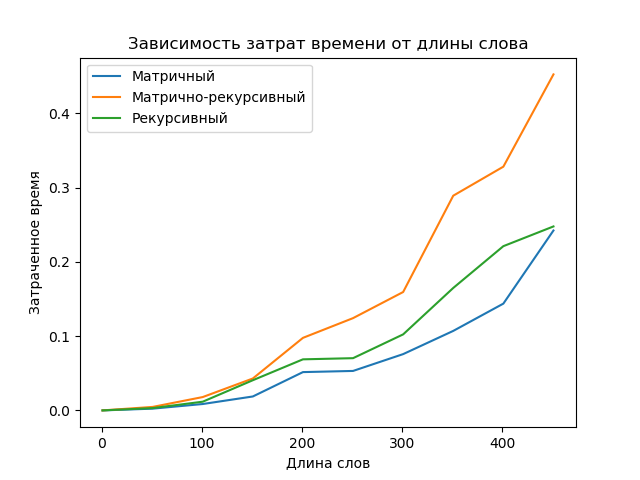
\includegraphics[width=0.7\linewidth]{src/Figure_1}
	\caption{График зависимости времени работы матричного, матрично-рекурсивного алгоритмов Левенштейна и матричного алгоритма Дамерау-Левенштейна от длины слов (ось абсцисс-время работы в секундах, ось ординат-длина слов)}
	\label{fig:figure1}
\end{figure}
По графику видно, что наиболее быстрым является матричный алгоритм поиска расстояния Левенштейна, несколько медленнее - матричный алгоритм поиска расстояния Дамерау-Левенштейна, что связано с более сложной логикой второго, и наиболее медленный - матрично-рекурсивный алгоритм, в связи с количеством дополнительных вызовов функции.\\
\begin{figure}[H]
	\centering
	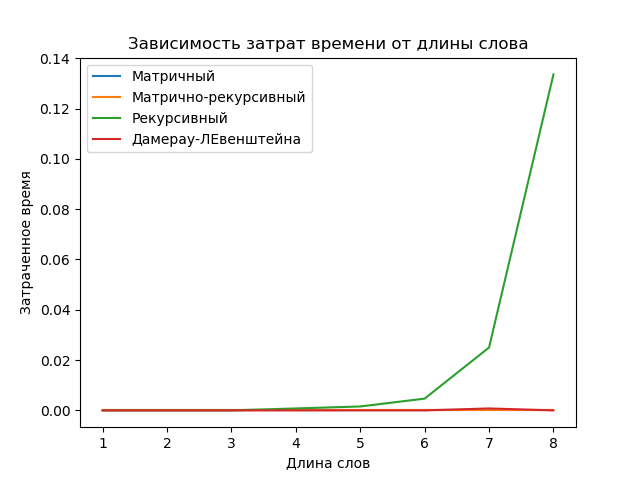
\includegraphics[width=0.7\linewidth]{src/Figure_2}
	\caption{График зависимости времени работы матричного, рекурсивного, матрично-рекурсивного алгоритмов Левенштейна и матричного алгоритма Дамерау-Левенштейна от длины слов (ось абсцисс-время работы в секундах, ось ординат-длина слов)}
	\label{fig:figure2}
\end{figure}
Время выполнения рекурсивного алгоритма увеличивается экспоненциально, в связи с чем итеративные или матрично-рекурсивные алгоритмы выполняются значительно быстрее.
\par Таким образом, самым быстрым алгоритмом оказался матричный алгоритм поиска расстояния Левенштейна, а самым медленным- рекурсивный. Можно сделать вывод, что матричный алгоритм эффективен для поиска редакционного расстояния для всех слов, но в случаях, когда ограничены ресурсы памяти и длина слов мала, лучше будет использовать рекурсивный алгоритм.
